% DATASETS

% d9f18e2 - DATASET FOR UNBOUNDED
% 2860d6fe - DATASET FOR HIGHSTART
% 53f6b74 - four levels for p_* - needed to examine lower bounds



% # Filter(Negate(is.factor),z[[gen]]) # quantile values for each combination of factor levels at gen
% # levels <- unique(interaction(Filter(is.factor,y))) # all unique combinations of factor levels in y


\chapter{Introduction}

In this section we explore the following research questions:

\vspace{0.3cm}
\begin{minipage}[l]{0.95\textwidth}
	\begin{enumerate}[label=RQ\arabic*:]
		\item Can inheritance emerge from simple selection and variation?
		\item Can evolution act on the inheritance mechanism to tune it for varying environmental conditions?
	\end{enumerate}
\end{minipage}
\vspace{0.3cm}

V+S-\textgreater{}I
Argument that heredity may in fact be a product of evolution rather than a precursor \autocite{Bourrat2015}

Heredity seen as method to maintain low entropy over much longer time than possible with non-biological systems: \quote{ Living systems can stay away from maximum entropy for much longer, indeed arbitrarily long (the biotic time scale is, for all we know, only limited by the existence of the biosphere). It is then this ability: to persist in a state of reduced entropy for biotic as opposed to abiotic time scales, that defines a set of molecules as living, and this set of molecules must achieve that feat via the self-replication of information.}{\autocite{Adami2015}}
	
``Context determines fitness'', where the environment is stable and affects the development of the entities

Degree of variation between generations important (no correlation means effectively unguided search, complete correlation means no source of novelties)

Problem is how can the optimal degree of variation (that is, inheritance) be established endogenously rather than as a model parameter?

Inheritance related to variation (between generations). Low variation implies high inheritance

Selection strengthens degree of inheritance

high fitness lineages more successful. Inheritance increases
correlation along lineage, so high fitness more likely to be passed
down. (Also low fitness, but they will suffer). On average then high
inheritance increases average fitness over time

\section{Assumptions}\label{assumptions}

No learning mechanisms--changes during lifetime

Corollary--if elements cannot change, then for population level change need to add or remove elements

\begin{itemize}
	\item
 If have no removals then population is either static (contradiction)
 or indefinitely expanding (practical problem)
	\item
 If have no additions, then cannot adjust population proportions
\end{itemize}

\section{Variation (and Inheritance)}\label{variation-and-inheritance}

Assume that variation occurs only on addition

\begin{itemize}
	\item
 If during life then, by definition, a learning mechanism
\end{itemize}

Corollary: no Lamarckian inheritance

Variation is in some element from parent to offspring

\begin{itemize}
	\item
 Degree of relationship interesting
	\item
 No relationship (no covariance) is as before--no learning
	\item
 If not related, then effectively random search--process is not
 `learning'--no information inheritance
	\item
 Duplication is effectively the same as just extending the lifespan -
 not interesting
	\item
 Somewhere in between (between 0 and 1) means heredity/inheritance
	\item
 Earlier work in biology has connected evolvability to mutation
 rate/inheritance rate
\end{itemize}

\section{Selection}\label{selection}

\subsection{Exogenous}\label{exogenous}

External calculation used directly to adjust population

Or guided evolution--external agency adjusts population directly

But as external element shared across population not evolvable

\subsection{Endogenous}\label{endogenous}

Feedback loop between element and everything else (in the sense of Pattee’s ``semantic
closure’’ discussed extensively in \autocite[sect. 3.5]{Taylor2001})

Causally results in a proportional change in population proportions

e.g., resource competition, or some other interaction between element and other things

Could occur on fixed timeframe (fixed generations, as common in biological modelling) or continuous

More generally, on range from \textasciitilde{}0 (continuous selection) to 1 (generations), although mid-points likely to be of little additional value

Affected by element and by everything else, so conceivably could be guided by modifying the environment in a calculated way

Reproduction follows from replication--no need to choose degree of similarity, emergent from lower level rules

\section{Hypothesis: Variation and Inheritance and Selection are sufficient for Evolution}\label{h1}

\begin{hypothesis}
	Variation and Inheritance and Selection are sufficient for Evolution, or V+S+I-\textgreater{}E
\end{hypothesis}\label{hypothesis-1}

From previous work\ldots{}

For some forms of V, S, I, E\ldots{}what are requirements?

\begin{itemize}
	\item
 For I, reasonable to define by degree--\autocite{Bourrat2015} = bias
 or degree of correlation between parent and offspring
	\item
 For S, compatible with resource competition--endogenous fitness
	\item
 For V, compatible with copy mutation
\end{itemize}

Can we construct a causal diagram from variation and selection that:

\begin{itemize}
	\item
 complies with requirement (optimizer, population dominated by best)
	\item
 less choice, more inevitable, less arbitrary
	\item
 foundation for creativity?
\end{itemize}

\section{Hypothesis: Correlated Variation and Selection are sufficient for Inheritance}\label{h2}

Inheritance comes from a copy mechanism under evolutionary control, such that the fidelity of the copy may
be varied by interaction with the environment.

Inheritance describes the similarity of an offspring to its parent, and depending on the context, can refer to the correlation for either a single trait or to a group of traits shared between offspring and parent (perhaps all of them.)

For the single trait case, when the correlation between the value for a parent's trait and an offspring's trait approaches the upper limit of 1.0 we say we have complete or full inheritance. Conversely, if there is no correlation (near the lower limit of 0) there is no inheritance and the entities are unrelated. We extend the measure to a group of traits simply by taking the average correlation of the group.

\begin{hypothesis}
	Variation, where there is some initial correlation between generations for a property, and Selection are sufficient for maximal Inheritance, or $V'+S\rightarrow I$
\end{hypothesis}\label{hypothesis-2}

\TODO{we mean inheritance increases to some optimal level}
Inheritance is defined as any correlation better than 0.5, or in other words, as better than chance. Fidelity is defined as the degree of correlation between parent and offspring values for the same trait.

\TODO{I iff V' (that is, with initial correlation)}
\TODO{Mechanism vs measure for fidelity}
\TODO{Can this be strengthened to include V+S necessary for I, or I-\textgreater{}V+S?}

\section{Predictions}\label{predictions}

In an unchanging environment, where the relative fitness of an entity, with respect to the environment, does not change over time, our expectations are:

\begin{enumerate}
	\item Average inheritance will tend towards perfect inheritance.
 Higher fitness entities will survive longer and reproduce more; higher fidelity reduces variation in fitness and so results in higher fitness being preferred.
	\item Population variance for inheritance will decrease more than chance.
\end{enumerate}

Under changing environmental conditions, where the fitness of an unchanging entity changes in response to environmental changes, we expect:

\begin{enumerate}
	\item The \gls{sd} of final fidelity under changing conditions \textgreater{} that under fixed conditions.
	\item The higher the variability in the environment, the higher the \gls{sd} of \emph{Fidelity}.
	\item \emph{Fidelity} at the end of a run under changing conditions \textless{} that under fixed conditions.
	\item The final \emph{Fitness} will be in the the range described by the distribution applied in the $tweakFitness$ function.
\end{enumerate}

\section{Alternative explanations}\label{alternative-explanations-1}

The three main alternatives, examined later in \cref{elimination-of-alternative-explanations} are:

\begin{enumerate}
	\item Variation alone is sufficient for Inheritance, or $V\rightarrow I$.
	\item Selection alone is sufficient for Inheritance, $S\rightarrow I$.
	\item Variation and Selection, without trait or property correlation, is sufficient for Inheritance.
\end{enumerate}

\chapter{Simulation model}

To test our hypothesis, we turn to simulation and experiment.

Simulation is a natural fit for the exploration of emergent systems where we expect complex behaviour from simple rules. 

If a simulation that accurately represents the system in the hypothesis behaves in a way that matches our predictions, the hypothesis is supported. On the other hand, if the behaviour doesn't align with the predictions, our hypothesis will be rejected.

Experimental tests are the strongest method we have to examine the claims made in hypothesis \autoref{hypothesis-2}. As explored earlier in \cref{the-legitimate-role-of-simulations}, logical argument or theorem-proving is difficult to apply to model-based systems. Thought experiments lack the strength we hope for, while experimentation is both feasible and, assuming correct design, rigorous.

Note that for those familiar with the design of experiments in the physical world, there are some differences in simulations, with the most significant being the sources and understanding of experimental errors. In simulation, experimental runs are exactly reproduceable, absent any dependency on factors external to the simulation. Variation is explictly introduced usually through a random number generator, which can be seeded to produce the same sequence of numbers again and again. This means that the practice in real-world experiments of ``blocking'' to control external variation is not required in simulation experiments. However, \gls{replicate}s where the same combination of factor values is run several times each with a different random seed value, remains valuable, but in this case less to control for experimental error and more to record the variation across a series of runs and the sensitivity of the model to parameter settings.

\section{Base model}\label{base-model}

All experiments in this part of the work make use of some variant of the same base model (\autoref{base-model-algorithm}) where the key elements of the hypothesis, such as inheritance fidelity, are represented as explicit parameters. The main elements will be quite familiar to anyone from Evolutionary Computation or Evolutionary Biology, although the introduction of fidelity is novel and important to the overall thesis.

We define a population of entities, each with two properties -- \emph{fitness} and \emph{fidelity} -- and a set of population-transforming functions.

\begin{itemize}
	\item \emph{Fitness} represents the probability that an entity will survive and possibly also reproduce, and has the usual range for a probability of $[0,1]$.
	\item \emph{Fidelity} measures the correlation between the child's value for a property and the same property's value in the parent. The range is $[0,1]$ where a value of $0$ means that the value for a child's property has no correlation with its parent's value for that property. High \emph{fidelity} values mean high correlation, and when $fidelity = 1.0$ the child's value is identical to the parent's.  There is a subtle difference between fidelity and inheritance: inheritance is the result, while fidelity is the mechanism, expressed as the degree of correlation between two generations. Inheritance can be thought of as emerging or resulting from fidelity.
\end{itemize}

The specific relationship between parent and child property values is given by a single mapping, represented in the algorithm by the function $Derive$.

The only transformation functions in the base model are for the two core elements from the hypothesis, \emph{Selection} and \emph{Variation}, although in later sections we will add others to examine the sensitivity of the model to various influences.

Each \gls{run} of the model consists of a fixed number of time steps (generations), where at each step the functions are applied in a defined order to the current population to form a replacement population. Colloquially, the replacement population is formed by a combination of parents from the current population, plus their children.

The model is parameterized (see \cref{tbl:parameter_definitions}) so that different combinations of factors can be investigated for their influence on the model's behaviour.

\begin{figure}[htb]
	\centering
	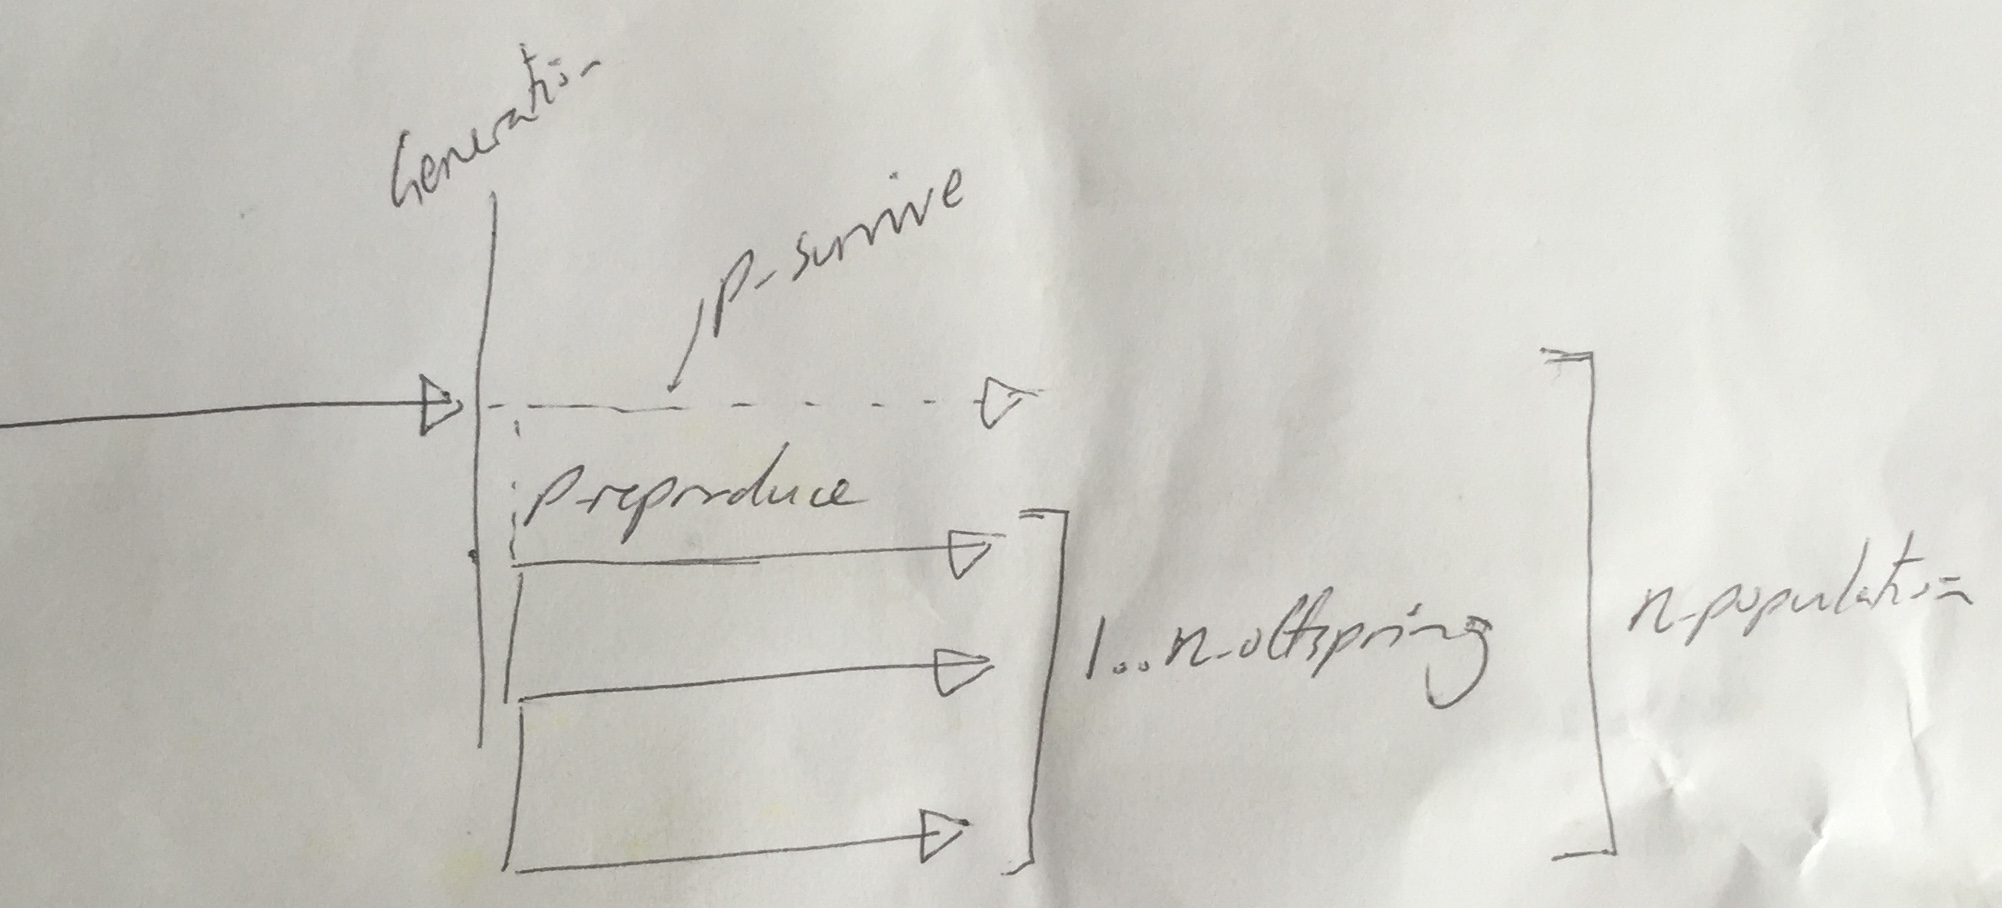
\includegraphics[width=0.95\linewidth]{figures/model}
\end{figure}

\begin{algorithm}
	\For{each generation $\in [1\dots$number of generations]}{
		$population\leftarrow Selection(population)$\;
		$population\leftarrow population \cup Variation(population)$\;
		\BlankLine
		\lIf{$population$ size is too small}{break}
	}
	\BlankLine
	\BlankLine
	\Def{Selection(population)}{
		$population_{new}\leftarrow \{\}$\;
		\For{each $entity \in population$} {
			\lIf{$p_{selection} = 0$}{$p\leftarrow $parent's fitness}
			\lElse{$p\leftarrow p_{selection}$}
			\Prob($p$:){
				Add $entity$ to $population_{new}$\;
			}
		}
		\Return $population_{new}$\;
	}
	\BlankLine
	\Def{Variation(population)}{
		$children\leftarrow \{\}$\;
		\For{each $entity$ in $population$}{
			\lIf{$p_{reproduce} = 0$} {$p\leftarrow $parent's fitness}
			\lElse{$p\leftarrow p_{reproduce}$}
			\BlankLine
			\Prob($p$:){
				\For{some number of children $\in \mathcal{U}[0,n_{children}]$} {
					$fitness\leftarrow$ Derive(parent's $fitness$, parent's $fidelity$)\;
					\uIf{Correlate Fidelity} {
						$fidelity\leftarrow$ Derive(parent's $fidelity$, parent's $fidelity$)\;
					}
					\uElse{
						$range\leftarrow$ some $x \in \mathcal{U}[0,1]$\;
						$fidelity\leftarrow$ Derive(parent's $fidelity$, $range$)\;
					}
					Create new $child$ with $fitness$ and $fidelity$\;
					Add $child$ to $children$\;
				}
			}
		}
		\Return $children$\;
	}
	\caption{Algorithm for the base model}\label{base-model-algorithm}
\end{algorithm}

\begin{figure}[ht]
	\centering
	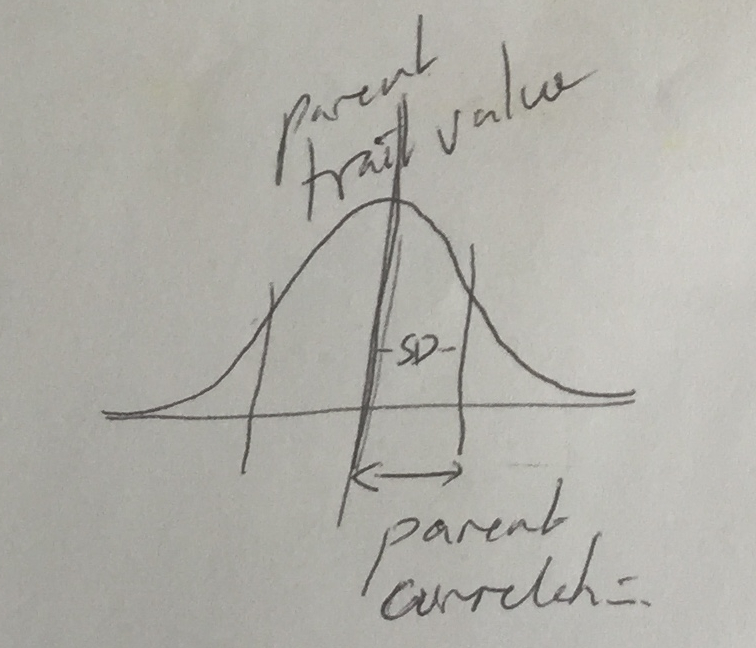
\includegraphics[width=0.95\linewidth]{figures/correlation}
\end{figure}

\begin{table}
	\begin{center}
		\caption{Model parameters}\label{tbl:parameter_definitions}
		\begin{tabular}{@{}llp{8cm}@{}}
			\toprule
			Parameter          & Value                                & Description                                                                                                                   \\
			\midrule
			$p_{reproduction}$ & $0$                                  & Probability of reproduction is given by the parent's $fitness$                                                                \\
                & $(0,1]$                              & Fixed probability of reproduction. The probability of reproduction for any entity is given by $p_{reproduction}$              \\
			$p_{selection}$    & $0$                                  & Probability of selection is given by the parent's $fitness$                                                                   \\
                & $(0,1]$                              & Probability of selection is unrelated to parent's $fitness$ and given instead by $p_{selection}$ for all entities             \\
			$n_{children}$     & $n_{children}\in \mathbb{Z}_{\ge 0}$ & Maximum number of children per parent                                                                                         \\
			%Restriction&			  	$(population, n)\mapsto population$&	Function to take $n$ elements from $population$\\
			Derive             & $[0,1]\times[0,1]\mapsto[0,1]$       & Function for generating a sample value $x$ from a distribution described by some measure of expected value and range          \\
			Correlate Fidelity & $\{\mathrm{true}, \mathrm{false}\}$  & Child's fidelity is related to parent's fidelity by parent's fidelity, or if false, by a random value $x\in \mathcal{U}[0,1]$ \\
			\bottomrule
		\end{tabular}
	\end{center}
\end{table}

\subsection{Claim of generality}

The model as described is general, under the assumptions given below. It is also directly comparable to models from Evolutionary Computation and so we also expect any results and conclusions to be relevant to EC models.

\TODO{Map to standard EA models - mutation only etc}

\section{Initial conditions and settings}\label{initial-conditions}

At the beginning of each run we construct an initial population to some design. Although a randomly chosen population is useful so as not to introduce any bias that may result from a consistent starting point, our interest is also in two other factors. First, under evolution we expect a general increase in fitness over time from any low initial starting point, and second, if a population is already in an evolved state with a reasonably high relative fitness we would not expect to see a decrease over time in fitness. We call these two initial starting points the low-start and High Start cases respectively, and they are described in the sections below.

\subsection{Low-start case}\label{low-start-case}

Entities in the low-start case begin with a low initial fidelity and fitness chosen randomly from a uniform distribution over a particular range (see \cref{tbl:ic}.) This case is of interest for two reasons: first, directly from hypothesis \autoref{hypothesis-2}, and driven by the overall goal of this thesis, we expect to see a population of low fidelity entities  eventually replaced by one of high (or at least higher) fidelity ones. Second, this is analogous to a key step on the path taken in biology from the abiotic world, where early copy mechanisms lacked the capabilities for high-fidelity copying (see earlier discussion in \cref{alternative-approaches}.)

\begin{table}[t]
	\begin{center}
		\caption{Initial conditions for low-start and High Start cases}\label{tbl:ic}
		\begin{tabular}{@{}lll@{}}
			\toprule
			Case                        & Property & Initial range           \\
			\midrule
			\multirow{2}{*}{Low-start}  & Fitness  & $\mathcal{U}[0, 0.3]$   \\
                         & Fidelity & $\mathcal{U}[0, 0.3]$   \\
			\midrule
			\multirow{2}{*}{High Start} & Fitness  & $\mathcal{U}[0, 0.9]$   \\
                         & Fidelity & $\mathcal{U}[0.5, 0.9]$ \\
			\bottomrule
		\end{tabular}
	\end{center}
\end{table}

\subsection{High-start case}\label{high-start-case}

In this case, entities start with a higher initial fidelity and a greater range of fitnesses (again, for specifics see \cref{tbl:ic}). This case examines the ability of the model to preserve advantageous entities, although, in the broader scope of the thesis, it is highly unlikely that any randomly created population would be of this initial form.

%In biological systems, random genetic drift can result in a decreasing fitness trend under certain circumstances \TODO{ref} but as our model omits drift \TODO{ true?} we can eliminate it as an acceptable explanation for any downwards trend.

\chapter{Initial screening}

Translating model parameters into factors in the experiment design results in the factors in the first column of \ref{tbl:factor-levels-for-investigation-into-inheritance-under-low-start-conditions}. As is usual with exploratory experiments with a number of parameters, where each run of the model has some cost in time or other resources, the key problem is to understand the relationship between parameters and response variables at an acceptable cost. In this case, our main cost is time - each run of an evolutionary model is cheap in resources but takes a little time. Exhaustively sampling the entire parameter space is unrealistic. Therefore, we first reduce the search space by limiting the number of values that each parameter can take. By choosing these values appropriately, we can construct an analysis model from the results that is sufficiently accurate for our exploratory purposes at a greatly reduced cost in time.

There are many approaches to this, but they mostly fall into two standard groups. First are response-surface methods which sample from the parameter space in a particular fashion to effectively construct an analysable function, or response-surface, from parameter values to response-variable values that approximates to some degree the behaviour of the model. The emphasis is on the shape of the response-surface; the parameter values are randomly chosen.

The usual alternative is some variant of a factorial design, where each parameter of interest is represented by a factor taking some small number of values, or levels (two levels being most common) and the analysis model constructed from runs that systematically work through a series of combinations of factors at different levels. The emphasis here is on the response given particular factor, and hence parameter, values.

\section{Experimental design}

As our interest is in the behaviour of the model both overall, and under specific conditions (such as the low-start case, or to the \emph{Correlate Fidelity} parameter), a factorial design is preferred.

Now, a full factorial design with seven 2-level factors would require testing $2^{7}$ combinations of factor values, or 128 sets of replicated runs, while a $2^{(7-3)}$ fractional factorial design \footnote{\eg  \url{http://www.itl.nist.gov/div898/handbook/pri/section3/eqns/2to7m3.txt}} can reduce this to 16 sets of replicated runs without loss of validity on the assumption that 3-factor interactions and higher are not significant. In other words, a $2^{(7-3)}$ design is sufficient to separate the main effect from any 2-factor interactions.  This seems a reasonable tradeoff between discriminatory power and the total number of runs required, given our exploratory goals.

The design is complicated a little by the suspicion that two factors - $p_{reproduction}$ and $p_{selection}$ - require more than two levels. Fortunately a $2^n$ fractional design can be extended relatively simply to include 4-level factors (\cite[368]{Montgomery2009}) either by replacement where each 4-level factor is mapped to two 2-level ones, or, as we choose to do, by a hybrid full-fractional design, where use combinations of our four-level factors,  $p_{reproduction}$ and $p_{selection}$, for two of the two-level factors, X1 and X2, of the standard $2^{(7-3)}$ design. This may not be quite as computationally efficient as a complete mixed-levels fractional factorial design but is efficient enough and meets our purposes.

We use a fractional factorial design to reduce the number of experimental runs required when compared to a full factorial design \autocite{Montgomery2009}. Although the number of runs is reduced, as each level of each factor occurs the same number of times in the results, the design remains ``balanced'' in the statistical sense, greatly easing analysis.

The number of \glspl{replicate} required for a particular statistical power is related to the \gls{sd} of the response variable.

\TODO{Based on preliminary runs, we begin with an initial estimate of 10 replicates for each combination of factor values given in the design; we confirm that this is sufficient through power calculations for specific tests where required in the later sections.}

\section{Factors and levels}\label{factors-and-levels}

Although several parameters in the model are continuous, at this stage the main ones can be reduced to a set of A/B alternatives, or two-level factors.

Of the others, $p_{reproduction}$ and $p_{selection}$ take four levels each to cover a reasonable range given the usual sensitivity of evolutionary models to these type of parameter; the value $0$ for the corresponding model parameter in each case means ``use parent's value'', and so is a special case. And as discussed in \ref{upper-size-bound}, \emph{Population Restriction} is held to Fitness-independent sampling.

The factors and levels used are given in \ref{tbl:factor-levels-for-investigation-into-inheritance-under-low-start-conditions}.

\begin{table}
	\begin{center}
		\caption{Factor levels for investigation into inheritance under low-start conditions}\label{tbl:factor-levels-for-investigation-into-inheritance-under-low-start-conditions}
		\begin{tabular}{@{}llp{6cm}@{}}
			\toprule
			Factor                 & Number of Levels & Levels                                                                                                                                              \\
			\midrule
			$p_{reproduction}$     & 4                & 0 or 0.33 or 0.66 or 1.0                                                                                                                            \\
			$p_{selection}$        & 4                & 0 or 0.33 or 0.66 or 1.0                                                                                                                            \\
			$n_{children}$         & 2                & 2 or 5                                                                                                                                              \\
			Population Restriction & 1                & Fitness-independent sampling                                                                                                                        \\
			Distribution           & 2                & Gaussian dist., $\mathbb{N}$ or Uniform dist., $\mathcal{U}$ \footnote{But see discussion in \ref{screening-distribution} as to the implementation} \\
			Correlate Fidelity     & 2                & false or true                                                                                                                                       \\
			\bottomrule
		\end{tabular}
	\end{center}
\end{table}

\section{Probability of selection and probability of reproduction}

We take these together as they interact. Where one or both parameters equal zero (use the parent's fitness as the probability of selection or probability of reproduction), the model is similar to a standard EA; any other value means selection or reproduction occurs with a fixed probability irrespective of fitness.

Why would we be interested in runs under these conditions? Imagine a run where selection has the value $1.0$ while reproduction takes value $0$ - parents always survive to the next generation (subject to any population limits naturally), while producing children at each generation with a probability proportional to their fitness. Or reverse these values ($p_{selection} = 0$ while $p_{reproduction} = 1.0$), giving a run where parents always produce a fixed number of $n_{offspring}$ children at each generation, but their own survival rate is proportional to their fitness.

The combination where both $p_{selection}$ and $p_{reproduction}$ are non-zero leads to uninteresting behaviour as the major source of variation has been removed from the model.

\section[Upper size bound]{Effect of upper bound on population size}\label{upper-size-bound}

In the absence of any restrictions on population size, there is nothing to prevent a population growing beyond the capacity of the simulation system. This is a practical problem rather than a property of the theoretical model, and so to have faith in the simulation and model it's important we eliminate the possibility of introducing bias to the results from the mechanism used to control population size.

The size of the population is driven by how population elements are introduced and removed. In standard Evolutionary Computation (\eg \cite[50]{DeJong2006}) the choice of strategy is important to the performance and outcomes of the algorithm. New elements can be straight replacements, like-for-like, of their parent, or be placed in competition against elements in the parent population, or completely replace the parent population. Elements may be removed as a result of selection, or through fitness-independent sampling to maintain a particular population size, or through some end-of-life calculation. The population size limit may act as both upper and lower bound on population size to maintain a specific size, or solely as upper bound.

Similar considerations apply to our model. Because we observe that the population size increases exponentially in many experimental runs (e.g., righthand side of \cref{fig:unboundedplot}), some upper bound on population size is needed. In the ``canonical'' Evolutionary Computation algorithm, a population limit results from selection where a set number of elements is extracted from the original population, with elements chosen by one of a wide range of selection algorithms (among many sources, see overviews in \cite[sect. 4.3.1]{DeJong2006} and \cite[sect. 4.2]{Vose:1999di}.) Here though we break the selection function from the population size limit in order to qualify the effect of the specific limiting mechanism used.

To summarize then, the goal of this section is to:

\begin{enumerate}
	\item Confirm that an upper bound on population size is required,
	\item Decide if the choice of method for maintaining the bound might significantly affect any conclusions from the hypothesis tests, and if it might,
	\item Determine which method to use for the remaining experiments.
\end{enumerate}

If there is an affect on the hypothesis tests attributable to the bound mechanism, then the conclusions from the test become contingent on the method. This reduces the scope somewhat, but without a change of investigative approach seems unavoidable.

\subsection{Effect of population limits}

% EXPERIMENT 1 - UNBOUNDED POPULATIONS


The environment is considered ``fixed'' (that is, each element's fitness value does not change); the initial population consists of 5000 elements constructed according to the low-start case (\cref{low-start-case}), and the model run with a maximum of 12 generations with

\begin{table} % d9f18e2
	\begin{center}
		\caption{Factor levels for investigation into the need for an upper-bound mechanism}
		\label{tbl:factors-levels-for-upper-bound-investigation}
		\begin{tabular}{@{}llp{6cm}@{}}
			\toprule
			Parameter              & Number of Levels & Levels                                                       \\
			\midrule
			$p_{reproduction}$     & 2                & 0 or 1.0                                                     \\
			$p_{selection}$        & 2                & 0 or 1.0                                                     \\
			$n_{children}$         & 2                & 2 or 5                                                       \\
			Population Restriction & 2                & No upper-bound, or Fitness-independent sampling              \\
			Distribution           & 2                & Gaussian dist., $\mathbb{N}$ or Uniform dist., $\mathcal{U}$ \\
			Correlate Fitness      & 2                & false or true                                                \\
			Correlate Fidelity     & 2                & false or true                                                \\
			Starting population    & 1                & Low-start settings                                           \\
			\bottomrule
		\end{tabular}
	\end{center}
\end{table}

\begin{knitrout}
\definecolor{shadecolor}{rgb}{0.969, 0.969, 0.969}\color{fgcolor}\begin{figure}[htp]
\includegraphics[width=\maxwidth]{generated_figures/unboundedplot-1} \caption[On the left, a histogram of number of generations achieved by an unbounded algorithm before either i) the population size increases beyond 10x the original population size, or ii) the simulation succeeds in reaching the expected number of generations (which never occurred in an unbounded population)]{On the left, a histogram of number of generations achieved by an unbounded algorithm before either i) the population size increases beyond 10x the original population size, or ii) the simulation succeeds in reaching the expected number of generations (which never occurred in an unbounded population). On the right, the growth of population size grouped by replicate (that is, by common factor levels) showing rapid population growth before reaching the 10x practicality limit.}\label{fig:unboundedplot}
\end{figure}


\end{knitrout}

Under these initial conditions, no experiment without an upper population bound continued for more than a handful of generations before the population size reached more than ten times the initial size. It is clear from \cref{fig:unboundedplot} that some form of upper bound is necessary.

\subsection[Choice of limit mechanism]{Is the choice of limit mechanism significant?}

Given then that an upper bound is needed for practicality, this section describes two possible approaches to the implementation of the \emph{Restriction} function in \ref{upper-bound-model-algorithm} and attempts to understand the form of the bias each introduces into the experimental results.

\begin{algorithm}
	\For{each generation $\in [1\dots$number of generations]}{
		$population\leftarrow Selection(population)$\;
		$population\leftarrow population \cup Variation(population)$\;
		$population\leftarrow Restriction(population)$\;
		\BlankLine
		\lIf{$population$ size is too small}{break}
	}
	\caption{Algorithm for the Model with an upper bound on population size. The \emph{Restriction} function is the only difference with the base model.}\label{upper-bound-model-algorithm}
\end{algorithm}

The first approach is to take a random sample of $n$ elements from the population, without regard for fitness (that is, fitness-independent sampling), while the other is to adopt the \emph{truncation} mechanism (described in \cite[124]{DeJong2006} alongside others) as representative (although strongly elitist) of a fitness-based mechanism (henceforth called fitness-based selection).

It might be argued that \emph{truncation} is too extreme to make a fair comparison. However, without an accepted scheme to order selection algorithms along a dimension of interest, such as selection pressure, it's hard to justify oversetting it by an alternative. The key criteria is whether the conclusions drawn from any particular algorithm can be extended to a more general conclusion, independent of the specifics of the algorithm or algorithms used. The specificity of selection algorithms means this a difficult argument to make, and most likely only possible by examining a number of them, which is beyond the scope of this work.

Returning then to our examination of fitness-independent and fitness-based upper bounds against the unlimited control case, the null, H$_0$, and alternative hypothesis, H$_1$, are as follows (examined for both population mean fitness and fidelity) :

\begin{itemize}[label={}]
	\item H$_0$: the two samples are drawn from the same continuous distribution
	\item H$_1$: the two samples are not drawn from the same continuous distribution
\end{itemize}

\subsubsection{Fitness-independent sampling}\label{fitness-independent-sampling}

The bound is implemented by a fitness-independent sampling of $n$ elements from the population (as given in the $Restriction$ function in \autoref{upper-bound-model-algorithm}), if and only if the pre-sampling population size is greater than $n$.

\begin{function}
	\SetKwProg{Def}{def}{:}{}
	\Def{Restriction(population,n)}{
		\Return $\text{random sample of }n\text{ elements from }population$\;
	}
	\caption{Restriction (Fitness-independent sampling)()}
\end{function}

%If we compare fitness-independent sampling to the control case without limits, we conclude that fitness independent sampling does indeed make a difference to the results, confirming the earlier visual assessment from the box and \gls{qq} plots (\cref{}.) This is somewhat unexpected as the average fitness before and after the application of the mechanism is, within sampling error, unchanged. It seems that the difference between limited and unlimited populations might come instead from the differences in population size in the selection and reproduction steps of the model rather than from any fitness-modifying actions of the restriction mechanism.

\subsubsection{Fitness-based selection}

The fitness-based population limit is based on \emph{truncation} from \cite[124]{DeJong2006}, chosen as it is reasonably representative of methods used in Evolutionary Algorithms, and as a highly-elitist algorithm should provide useful contrast to the effectively uniform mechanism of \cref{fitness-independent-sampling}. If the two mechanisms produce similar results then it might be argued that other mechanisms are likely to be similar also.

It also recognizes that in both Evolutionary Computation and natural populations, the population limit is a function of the carrying capacity of the environment and fitness determines the selection.

\begin{function}
	\SetKwProg{Def}{def}{:}{}
	\Def{Restriction(population,n)}{
		$sortedPopulation\leftarrow$ sorted population by element fitness, in decreasing order \;
		\Return $\text{first }n\text{ elements from }sortedPopulation$\;
	}
	\caption{Restriction (Fitness-based selection)()}
\end{function}

\subsection{Experimental design}

% EXPERIMENT 2 - CHOICE OF LIMIT MECHANISM


\begin{table} % 53f6b74
	\begin{center}
		\caption{Factor levels for the choice of an upper-bound mechanism}
		\label{tbl:factor-levels-for-the-choice-of-an-upper-bound-mechanism}
		\begin{tabular}{@{}llp{6cm}@{}}
			\toprule
			Parameter              & Number of Levels & Levels                                                       \\
			\midrule
			$p_{reproduction}$     & 4                & 0 or 0.33 or 0.66 or 1.0                                     \\
			$p_{selection}$        & 4                & 0 or 0.33 or 0.66 or 1.0                                     \\
			$n_{children}$         & 2                & 2 or 5                                                       \\
			Population Restriction & 2                & Fitness-independent sampling, or Fitness-based selection     \\
			Distribution           & 2                & Gaussian dist., $\mathbb{N}$ or Uniform dist., $\mathcal{U}$ \\
			Correlate Fitness      & 2                & false or true                                                \\
			Correlate Fidelity     & 2                & false or true                                                \\
			\bottomrule
		\end{tabular}
	\end{center}
\end{table}



Data is from 640 runs -- 64 unique sets of factors, each with 10 replicates -- with settings given in \cref{tbl:factor-levels-for-the-choice-of-an-upper-bound-mechanism} under fixed conditions, of which we are exclusively concerned with the subset of 604 runs that reached completion at 500 generations.

\subsection{Results and discussion}

The runs that reached completion are evenly distributed between the two methods, fitness-independent (300 runs) and fitness-based (304 runs), indicating that the two methods at least appear comparable with respect to their affect on population size.

\begin{knitrout}
\definecolor{shadecolor}{rgb}{0.969, 0.969, 0.969}\color{fgcolor}\begin{figure}[htp]
\includegraphics[width=\maxwidth]{generated_figures/limitcomparisonplots-1} \caption[Summary plots for fitness-independent sampling ("Independent") and fitness-based or dependent selection ("Dependent"), where the top line contains density plots and the bottom line boxplots showing ranges for both final mean fidelity (on the left-hand side) and final mean fitness (on the right)]{Summary plots for fitness-independent sampling ("Independent") and fitness-based or dependent selection ("Dependent"), where the top line contains density plots and the bottom line boxplots showing ranges for both final mean fidelity (on the left-hand side) and final mean fitness (on the right).}\label{fig:limitcomparisonplots}
\end{figure}


\end{knitrout}

\begin{knitrout}
\definecolor{shadecolor}{rgb}{0.969, 0.969, 0.969}\color{fgcolor}\begin{figure}[htp]
\includegraphics[width=\maxwidth]{generated_figures/limitqqplots-1} \caption[\Gls{qq} plots comparing fitness-independent and fitness-based or dependent results for fidelity (left) and fitness (right)]{\Gls{qq} plots comparing fitness-independent and fitness-based or dependent results for fidelity (left) and fitness (right).}\label{fig:limitqqplots}
\end{figure}


\end{knitrout}

%Standard non-parametric tests include Wilcoxon and Mann-Whitney for comparing two
%independent continuous random samples where the underlying distributions
%are known to have essentially the same shape, or a Friedman test where the samples might be related (\eg in block %experiment designs) and the objective is to distinguish differences between treatments.



Applying a two-sample Kolmogorov-Smirnov test to determine if the results for each method are taken from the same distribution provides strong evidence (for population mean fidelity, approx. p-value=0 and for pop. mean fitness, approx. p-value=0) to reject the null hypothesis, confirmed by visual inspection of \cref{fig:limitcomparisonplots} and \cref{fig:limitqqplots}. The distributions produced by the two methods are different for both average fidelity and average fitness.

From these tests it is clear that the two methods do not have statistically similar effects for both fidelity and fitness, and hence we cannot find support for the contention that our conclusions in the hypothesis tests can be made without extensive consideration of limit method. Method is important, and our conclusions are dependent on the method chosen.

This conclusion of course is based on a comparison of two particular methods; a third, fitness-based, method may produce distributions that are statistically similar to those of, say, sampling. In which case we might conclude that any conclusions drawn on the basis of sampling would also extend to this third method. This extension however is left for future work.

Returning to our goal, as the choice of method affects our results and for practical reasons we must make a choice, it seems reasonable to choose a method that has as small an influence as possible on the conclusions we draw from our hypothesis tests. As our tests involve fitness, a method that is by design orthogonal to fitness is the better choice. A sampling method is a better fit for this than a selection method, which biases on fitness, and therefore we adopt fitness-independent sampling rather than fitness-based restriction.

\section[Lower size bound]{Lower limit on population size}\label{lower-size-limit}

% EXPERIMENT - Lower size bound



\begin{table} % 53f6b74
	\begin{center}
		\caption{Factor levels for the choice of a lower-bound mechanism}
		\label{tbl:factor-levels-for-the-choice-of-a-lower-bound-mechanism}
		\begin{tabular}{@{}llp{6cm}@{}}
			\toprule
			Parameter              & Number of Levels & Levels                                                       \\
			\midrule
			$p_{reproduction}$     & 4                & 0 or 0.33 or 0.66 or 1.0                                     \\
			$p_{selection}$        & 4                & 0 or 0.33 or 0.66 or 1.0                                     \\
			$n_{children}$         & 2                & 2 or 5                                                       \\
			Population Restriction & 2                & Fitness-independent sampling, or Fitness-based selection     \\
			Distribution           & 2                & Gaussian dist., $\mathbb{N}$ or Uniform dist., $\mathcal{U}$ \\
			Correlate Fitness      & 2                & false or true                                                \\
			Correlate Fidelity     & 2                & false or true                                                \\
			\bottomrule
		\end{tabular}
	\end{center}
\end{table}

We now turn to the other bound, and the impact of population extinctions. Runs in which the population dies out are incompatible with ongoing evolution, and so should be separated from other, sustainable, runs in the analysis. This situation does arise in our simulation: not all runs in the experiment described in \ref{upper-size-bound} completed the target of 500 generations (\cref{fig:popoverall}), and of those that did, not all completed with a sustainable population size.

\begin{knitrout}
\definecolor{shadecolor}{rgb}{0.969, 0.969, 0.969}\color{fgcolor}\begin{figure}[htp]
\includegraphics[width=\maxwidth]{generated_figures/popoverall-1} \caption[Not all runs in fixed conditions can maintain a substantial population size over time]{Not all runs in fixed conditions can maintain a substantial population size over time. The horizontal line at the top of the figure is from runs that were capped by the population upper-bound, while the great majority of unsustainable runs fall within the asymptotically decreasing band from top-left to bottom-right. Note the extreme case represented by the almost vertical set of points to the far left, discussed in the text.}\label{fig:popoverall}
\end{figure}


\end{knitrout}

Of the 320 experiment runs, 20 fail to reach completion, and 10 complete with a population size substantially smaller ($\leq$ 138) than the population size in the other completed runs. In fact, all other runs reach completion with a population size at the upper bound limit of 5000.

From the clustering evident in \ref{fig:popoverall} we assert that the experiment runs can be separated into two disjoint sets - those that reach completion with a population size at or very near the upper-size limit, and those whose population is tending towards zero. Our interest lies only in sustainable populations and therefore from here on we exclude all runs where the population does not reach completion at or near the upper-size limit, without loss of generality.

%Inspecting the results by factor:
%\begin{enumerate}
%	\item All runs with $p_{reproduction}=0.33$ and $n_{children}=2$ fail to complete.
%	\item All runs that complete, but with an unsustainably small population, also include $p_{selection}=0.66$.
%\end{enumerate}
%
%To conclude this brief examination of lower-bounds, runs with factors associated with population extinction ($p_{reproduction}=0.33$, $n_{children}=2$ and $p_{selection}=0.66$) will be omitted from further analysis.

\TODO{explanation for extreme left case}

Note that these results also provide support for an experiment duration of 500 generations - either a run maintains a stable population (and so the duration is unrelated to population size considerations), or if a population is to go extinct it does so by 500 generations or soon after and so can easily be identified for special treatment.

\section{Number of offspring}


\begin{table} % 53f6b74
	\begin{center}
		\caption{Factor levels for the investigation into number of offspring}
		\begin{tabular}{@{}llp{6cm}@{}}
			\toprule
			Parameter              & Number of Levels & Levels                                                       \\
			\midrule
			$p_{reproduction}$     & 4                & 0 or 0.33 or 0.66 or 1.0                                     \\
			$p_{selection}$        & 4                & 0 or 0.33 or 0.66 or 1.0                                     \\
			$n_{children}$         & 2                & 2 or 5                                                       \\
			Population Restriction & 2                & Fitness-independent sampling, or Fitness-based selection     \\
			Distribution           & 2                & Gaussian dist., $\mathbb{N}$ or Uniform dist., $\mathcal{U}$ \\
			Correlate Fitness      & 2                & false or true                                                \\
			Correlate Fidelity     & 2                & false or true                                                \\
			\bottomrule
		\end{tabular}
	\end{center}
\end{table}

\begin{knitrout}
\definecolor{shadecolor}{rgb}{0.969, 0.969, 0.969}\color{fgcolor}\begin{figure}[htp]
\includegraphics[width=\maxwidth]{generated_figures/popoffspring-1} \caption[Population size over time for two values of parameter ]{Population size over time for two values of parameter $n_{children}$ - 2 (on the left) and 5 (on the right) .}\label{fig:popoffspring}
\end{figure}


\end{knitrout}

The vertical line on the extreme left of the right-hand side facet of \cref{fig:popoffspring} (for $n_{offspring} = 5$) consists of 58 runs from a total of nrow(subset(df,gen==0)) where the population dropped in the first generation to a mean size of 2855.25, before recovering to the population upper limit by generation 4. This is a characteristic of the initial conditions: runs where $n_{offspring} = 2$ and the probability of reproduction or selection is low, either because the parameter has a low, fixed, value or because they are derived from the parent's value, suffer high selection and low reproduction initially. Taking the case where both are given by the parent's value,  the initial values are defined by the low-start case and $p_{reproduction} = p_{selection} = $0.1500929. The difference between the two facets can be explained by the higher reproduction rate in the right-hand facet.

A similar effect can be seen in the left-hand side facet for $n_{offspring} = 2$ where some of the affected runs recovered while others went to extinction.

\section{Fidelity correlation}

\emph{Fidelity correlation} is parameterized in order to test the hypothesis that correlation is required for inheritance; the alternative hypothesis that inheritance can arise without correlation corresponds to \emph{Fidelity correlation} being false.

\section{Derive parameter}\label{screening-distribution}


\begin{table} % 53f6b74
	\begin{center}
		\caption{Factor levels for the investigation of Derive}
		\begin{tabular}{@{}llp{6cm}@{}}
			\toprule
			Parameter              & Number of Levels & Levels                                                       \\
			\midrule
			$p_{reproduction}$     & 4                & 0 or 0.33 or 0.66 or 1.0                                     \\
			$p_{selection}$        & 4                & 0 or 0.33 or 0.66 or 1.0                                     \\
			$n_{children}$         & 2                & 2 or 5                                                       \\
			Population Restriction & 2                & Fitness-independent sampling, or Fitness-based selection     \\
			Distribution           & 2                & Gaussian dist., $\mathbb{N}$ or Uniform dist., $\mathcal{U}$ \\
			Correlate Fitness      & 2                & false or true                                                \\
			Correlate Fidelity     & 2                & false or true                                                \\
			\bottomrule
		\end{tabular}
	\end{center}
\end{table}

\begin{knitrout}
\definecolor{shadecolor}{rgb}{0.969, 0.969, 0.969}\color{fgcolor}
\includegraphics[width=0.45\linewidth]{generated_figures/gaussian-1} 
\includegraphics[width=0.45\linewidth]{generated_figures/gaussian-2} 

\end{knitrout}

The \emph{Derive} parameter describes a function to return a value in the range $[0,1]$ given two parameters, also in the range $[0,1]$. Obvious candidates for \emph{Derive} include probability distributions, where the function samples a value from a distribution. If the distribution is gaussian, the two parameters to \emph{Derive} would describe its mean and variance.  

From a visual inspection, we conclude that the results appear very similar for Uniform and Gaussian distributions.

\section{Conclusions}

Independent variable is Fidelity correlation, the main factor of interest from hypothesis

Dependent variables, to qualify the sensitivity of the model:
\begin{enumerate}
	\item Distribution
	\item Number of offspring
\end{enumerate}

Set remaining parameters based on these screening experiments:
\begin{enumerate}
	\item Upper-size bound - sampling % truncate == 0
	\item Lower-size bound - sustainable populations % gen for run == max gen, and pop at max gen > 1000
	\item Probabilities - at least one of $p_{reproduction}$ and $p_{selection}$ is related to the parent's fitness (\ie the factor level has the special case value of 0.) % 
	      	
 % All runs that complete - that is, where gen == max(df$gen) & pop > 1000 or subset(df,gen==500 & pop>1000)
 % runs <- subset(df, gen==max(df$gen) & pop>1000)[,'run']
 % subset(df, truncate == 0 & run %in% runs & (p_reproduce==0 | p_selection == 0))
 % Use subset(df,correlation_correlation==1) by hypothesis, correlation_correlation==0 is control
	      	
\end{enumerate}

\chapter[Test under fixed conditions]{Experimental test of hypothesis under fixed conditions}\label{experimental-test-of-h2-under-fixed-conditions}

Returning to the overall goals for these experiments (to test the predictions of hypothesis \autoref{hypothesis-2}, and to examine the impact of the factors on the results), hypothesis \autoref{hypothesis-2} makes two predictions for fixed environments:

\begin{enumerate}
	\item Average inheritance will tend towards perfect inheritance, and
	\item Population variance for inheritance will decrease more than chance.
\end{enumerate}

The low-start case is the most significant as it describes the core of the thesis - that good quality inheritance can develop from imperfect beginnings, such as could occur in the emergence of artificial evolution, or indeed as might be found during the transition from non-living to life. This makes it a key step along the way towards the evolution of artifical evolution, the main subject of this thesis.

The first test therefore is to examine if inheritance emerges from low-fidelity and low-fitness initial conditions \cref{inheritance-low-start} and confirm that it is maintained under high-start conditions \cref{inheritance-high-start}, and then finally test whether the population variance for inheritance decreases as predicted \cref{sd-low-start}.

\section{Emergence of inheritance from low-start initial conditions}\label{inheritance-low-start}

As discussed earlier in \cref{synthesis-from-a-general-evolutionary-model}, inheritance is the outcome of the relationship between parent and child traits, as represented by the measure of fidelity.

% EXPERIMENT 3 - Fidelity approaches 1.0

We start with the following null and alternative hypotheses:

\begin{itemize}[label={}]
	\item H$_0$: fidelity does not approach 1.0 during a run, irrespective of factor values, or \newline
 $\vert \overline{fidelity}_{end}-\overline{fidelity}_{start} \vert = 0$
	\item H$_1$: fidelity increases to near 1.0 during a run, for some factor values, or \newline
 $\overline{fidelity}_{end}-\overline{fidelity}_{start} > 0$ and $1.0-\overline{fidelity}_{end} < \delta$ for some $\delta$ and for some factor values.
\end{itemize}

\subsection{Response variables}\label{response-variables}

From the predictions of the hypothesis (\cref{predictions}), the main property of interest is \emph{fidelity}, or the correlation between parent and child property values. \emph{Fidelity} therefore is our response variable.
\\

Specifically we use $\overline{fidelity}_{end}$, or the mean value for \emph{fidelity} (across all replicates) at the end of a run, as under hypothesis \autoref{hypothesis-2} we expect $\overline{fidelity}_{end}$ to approach 1.0 in an unchanging environment.

\subsection{Design}\label{design}



\begin{table} % 5e33a27 and 819350e
	\begin{center}
		\caption{Factor levels for testing the hypothesis prediction of perfect inheritance in unchanging conditions}
		\begin{tabular}{@{}llp{6cm}@{}}
			\toprule
			Parameter              & Number of Levels & Levels                                                   \\
			\midrule
			$p_{reproduction}$     & 2                & 0 or 0.66                                                \\
			$p_{selection}$        & 2                & 0 or 0.66                                                \\
			$n_{children}$         & 2                & 2 or 5                                                   \\
			Population Restriction & 2                & Fitness-independent sampling or fitness-based truncation \\
			Distribution           & 2                & Gaussian dist., $\mathbb{N}$ or folded Gaussian          \\
			Correlate Fidelity     & 2                & false or true                                            \\
			Shape of environment change		2&	Abrupt or continuous\\
			\bottomrule
		\end{tabular}
	\end{center}
\end{table}

\begin{knitrout}
\definecolor{shadecolor}{rgb}{0.969, 0.969, 0.969}\color{fgcolor}\begin{figure}[htp]
\includegraphics[width=\maxwidth]{generated_figures/lowstart-1} \caption{Summary results for low-start case, showing on the left-hand side an overview for the final mean fidelity ($\overline{fidelity}_{end}$) for each run and a density plot showing the distribution of $\overline{fidelity}_{end}$. The right-hand side shows the corresponding plots for final mean fitness ($\overline{fitness}_{end}$)}\label{fig:lowstart}
\end{figure}


\end{knitrout}

\begin{knitrout}
\definecolor{shadecolor}{rgb}{0.969, 0.969, 0.969}\color{fgcolor}\begin{figure}[htp]
\includegraphics[width=\maxwidth]{generated_figures/lowstartbyfactor-1} \caption[Summary for low-start, this time averaged across all replicates of each factor combination (that is, grouped by replicate)]{Summary for low-start, this time averaged across all replicates of each factor combination (that is, grouped by replicate). Dark-coloured points represent values at end of run; light-coloured points are for initial values. Missing points are from those replicates that did not complete.}\label{fig:lowstartbyfactor}
\end{figure}


\end{knitrout}



\begin{knitrout}
\definecolor{shadecolor}{rgb}{0.969, 0.969, 0.969}\color{fgcolor}\begin{figure}[htp]
\includegraphics[width=\maxwidth]{generated_figures/highstart-1} \caption{Summary results for high-start case, showing on the left-hand side an overview for the final mean fidelity ($\overline{fidelity}_{end}$) for each run and a density plot showing the distribution of $\overline{fidelity}_{end}$. The right-hand side shows the corresponding plots for final mean fitness ($\overline{fitness}_{end}$)}\label{fig:highstart}
\end{figure}


\end{knitrout}

\begin{knitrout}
\definecolor{shadecolor}{rgb}{0.969, 0.969, 0.969}\color{fgcolor}\begin{figure}[htp]
\includegraphics[width=\maxwidth]{generated_figures/highstartbyfactor-1} \caption[Summary for high-start, averaged across all replicates for each combination of factors, as seen earlier in the low-start case]{Summary for high-start, averaged across all replicates for each combination of factors, as seen earlier in the low-start case. Light-coloured points for initial state and dark-coloured ones for final values.Missing points are from replicates that did not complete.}\label{fig:highstartbyfactor}
\end{figure}


\end{knitrout}

\subsection{Results and discussion}

Our interest is in the final values for fidelity under fixed-environment, low-start, conditions. Therefore, data is from the final generation of those fixed-environment runs that reached completion at generation 500 from the low-start dataset; a total of 80 runs out of the full dataset of 640 runs.

A simple visual inspection of this data in \cref{fig:lowstart} reveals that the fidelity measure is distinctly bimodal, with peaks around final mean fidelity values 0.5--0.6 and 1.0. Fitness is also bimodal, but less so than fidelity. From inspection, it seems clear that fidelity does approach 1.0 for some combination of factor levels.

\begin{knitrout}
\definecolor{shadecolor}{rgb}{0.969, 0.969, 0.969}\color{fgcolor}\begin{figure}[htp]
\includegraphics[width=\maxwidth]{generated_figures/lowstartfactors-1} \caption[Comparison between correlated and uncorrelated factors in the low-start case for the factor \textbf{Correlate Fidelity} showing results for final mean fidelity (]{Comparison between correlated and uncorrelated factors in the low-start case for the factor \textbf{Correlate Fidelity} showing results for final mean fidelity ($\overline{fidelity}_{end}$, on the left) and final mean fitness ($\overline{fitness}_{end}$, on right)}\label{fig:lowstartfactors}
\end{figure}


\end{knitrout}

From \cref{fig:lowstartbyfactor}, all runs result in an increase in fidelity from the initial range of $[0, 0.3]$ but only some approach or reach 1.0. Those that do are uniformly associated with the \textbf{Correlate Fidelity} factor value of \emph{true} (see top-left plot in \cref{fig:lowstartfactors}), and those that did not had a \textbf{Correlate Fidelity} value of -1.

In conclusion, H$_0$ can be rejected, and H$_1$ accepted. Inheritance increases regardless of the model design, but is strongest when \textbf{Correlate Fidelity} is \emph{true}, that is, when the child's fidelity is correlated with that of its parent.

\section{Confirmation of inheritance under high-start conditions}\label{inheritance-high-start}

\TODO{Experiment settings}

% EXPERIMENT 4 - Inheritance under high-start conditions


\begin{table} % 5e33a27 and 819350e
	\begin{center}
		\caption{Factor levels for confirmation of hypothesis prediction under high-start initial conditions}
		\begin{tabular}{@{}llp{6cm}@{}}
			\toprule
			Parameter              & Number of Levels & Levels                                                   \\
			\midrule
			$p_{reproduction}$     & 2                & 0 or 0.66                                                \\
			$p_{selection}$        & 2                & 0 or 0.66                                                \\
			$n_{children}$         & 2                & 2 or 5                                                   \\
			Population Restriction & 2                & Fitness-independent sampling or fitness-based truncation \\
			Distribution           & 2                & Gaussian dist., $\mathbb{N}$ or folded Gaussian          \\
			Correlate Fidelity     & 2                & false or true                                            \\
			Shape of environment change		2&	Abrupt or continuous\\
			\bottomrule
		\end{tabular}
	\end{center}
\end{table}

\begin{knitrout}
\definecolor{shadecolor}{rgb}{0.969, 0.969, 0.969}\color{fgcolor}\begin{figure}[htp]
\includegraphics[width=\maxwidth]{generated_figures/highstartfactors-1} \caption{Comparison between correlated and uncorrelated factors in the high-start case for the factor \textbf{Correlate Fidelity}. As before, results for final mean fidelity ($\overline{fidelity}_{end}$) are on the left, and for final mean fitness ($\overline{fitness}_{end}$) on the right.}\label{fig:highstartfactors}
\end{figure}


\end{knitrout}

\section{Variance of Fidelity reduces under low-start conditions}\label{sd-low-start}

% EXPERIMENT 5 - SD of Fidelity approaches 0

The second prediction of the hypothesis is that population variance for inheritance ($\sigma_{fidelity}$) should decrease over time towards a limit of $0$ in fixed environments.

\begin{itemize}[label={}]
	\item H$_0$: $\sigma_{fidelity_{end}}-\sigma_{fidelity_{start}} >= 0$, for all factor values.
	\item H$_1$: $\sigma_{fidelity_{end}}-\sigma_{fidelity_{start}} < 0$, for some factor values.
\end{itemize}

We use the same experimental setup and data as for the first hypothesis test in \cref{tbl:factor-levels-for-investigation-into-inheritance-under-low-start-conditions}.



\begin{table} % 5e33a27 and 819350e
	\begin{center}
		\caption{Factor levels for testing the hypothesis prediction that the population variance of inheritance should reduce to nothing in unchanging environments}
		\begin{tabular}{@{}llp{6cm}@{}}
			\toprule
			Parameter              & Number of Levels & Levels                                                   \\
			\midrule
			$p_{reproduction}$     & 2                & 0 or 0.66                                                \\
			$p_{selection}$        & 2                & 0 or 0.66                                                \\
			$n_{children}$         & 2                & 2 or 5                                                   \\
			Population Restriction & 2                & Fitness-independent sampling or fitness-based truncation \\
			Distribution           & 2                & Gaussian dist., $\mathbb{N}$ or folded Gaussian          \\
			Correlate Fidelity     & 2                & false or true                                            \\
			Shape of environment change		2&	Abrupt or continuous\\
			\bottomrule
		\end{tabular}
	\end{center}
\end{table}

\subsection{Results and discussion}

\begin{knitrout}
\definecolor{shadecolor}{rgb}{0.969, 0.969, 0.969}\color{fgcolor}\begin{figure}[htp]
\includegraphics[width=\maxwidth]{generated_figures/lowstartranges1-1} \caption[Smoothed ranges over time of the standard deviation of fidelity (top) and fitness (bottom) for all levels of all factors, broken out by level of \emph{Correlate Fidelity}]{Smoothed ranges over time of the standard deviation of fidelity (top) and fitness (bottom) for all levels of all factors, broken out by level of \emph{Correlate Fidelity}. Lines that drop below zero are an artifact of the line smoothing algorithm used (local polynomial regression fitting).}\label{fig:lowstartranges1}
\end{figure}


\end{knitrout}

\begin{knitrout}
\definecolor{shadecolor}{rgb}{0.969, 0.969, 0.969}\color{fgcolor}\begin{figure}[htp]
\includegraphics[width=\maxwidth]{generated_figures/lowstartranges2-1} \caption[Smoothed ranges for the mean rather than the standard deviation - mean fidelity on the top row, mean fitness below - again by \emph{Correlate Fidelity}]{Smoothed ranges for the mean rather than the standard deviation - mean fidelity on the top row, mean fitness below - again by \emph{Correlate Fidelity}.}\label{fig:lowstartranges2}
\end{figure}


\end{knitrout}

Data is all generations for those fixed-environment runs that reached completion with a 'sustainable' population (see \cref{lower-size-limit}) at generation 500; 80 runs out of the full dataset of 640 runs.

%<<lowstartranges2, pdfcrop=TRUE, echo=FALSE, cache=TRUE, fig.pos='htp', fig.cap='Range of 25\\% to 75\\% quartiles for \\gls{sd} for \\emph{true} setting for factor \\textbf{Correlate Fidelity}'>>=
%z<-by(df,df$gen,function(x) {aggregate(x$sd_cor ~ x$correlation_correlation, data=x, quantile)}) # quantiles aggregated by correlation_correlation
%z1<-apply(z,1,function(x){c(x[[1]][[2]][[2,2]],x[[1]][[2]][[2,3]],x[[1]][[2]][[2,4]])}) # correlation_correlation == -1
%z1<-apply(z,1,function(x){c(x[[1]][[2]][[1,2]],x[[1]][[2]][[1,3]],x[[1]][[2]][[1,4]])}) # correlation_correlation == 1
%z2<-z1[1:3,1:501]
%z3<-as.data.frame(cbind(1:501,z2[1,],z2[2,],z2[3,]))
%ggplot(z3,aes(V1,V2,V3)) + geom_ribbon(data=z3,aes(ymin=V2,ymax=V4), alpha = 0.2) + geom_line(aes(V1,V3))
%@

\section{Confirmation that variance decreases under high-start conditions}

% EXPERIMENT 6 - SD of Fidelity approaches 0



\begin{table} % 5e33a27 and 819350e
	\begin{center}
		\caption{Factor levels for confirmation that variance also decreases under high-start conditions}
		\label{Factor-levels-for-investigation-into-variance-under-high-start-conditions}
		\begin{tabular}{@{}llp{6cm}@{}}
			\toprule
			Parameter              & Number of Levels & Levels                                                   \\
			\midrule
			$p_{reproduction}$     & 2                & 0 or 0.66                                                \\
			$p_{selection}$        & 2                & 0 or 0.66                                                \\
			$n_{children}$         & 2                & 2 or 5                                                   \\
			Population Restriction & 2                & Fitness-independent sampling or fitness-based truncation \\
			Distribution           & 2                & Gaussian dist., $\mathbb{N}$ or folded Gaussian          \\
			Correlate Fidelity     & 2                & false or true                                            \\
			Shape of environment change		2&	Abrupt or continuous\\
			\bottomrule
		\end{tabular}
	\end{center}
\end{table}

\subsection{Response variables}

The main response variable is the standard deviation of fidelity.

\subsection{Initial conditions}

Initial conditions are given in \cref{Factor-levels-for-investigation-into-variance-under-high-start-conditions}.

\subsection{Results and discussion}

\begin{knitrout}
\definecolor{shadecolor}{rgb}{0.969, 0.969, 0.969}\color{fgcolor}\begin{figure}[htp]
\includegraphics[width=\maxwidth]{generated_figures/ExperimentVarianceUnderHighStart-1} \caption[High start case]{High start case: smoothed ranges for standard deviation of fidelity, as before grouped by \emph{Correlate Fidelity}.}\label{fig:ExperimentVarianceUnderHighStart}
\end{figure}


\end{knitrout}

%\section{Factor interactions}
%% EXPERIMENT 7 - Factor significance
%% Dataset: 2860d6fe
%
%<<ExperimentFactorInteractions, pdfcrop=TRUE, echo=FALSE, cache=TRUE>>=
%temp <- load.results('results/results-819350e.data')
%temp <- subset(temp, environment_change_frequency == 0 & truncate==0 & correlation_correlation==1)
%completing_factors <- unique(interaction(Filter(is.factor,temp[temp$gen==500,]))) # the factor levels that resulted in 500 generations
%df <- temp[interaction(Filter(is.factor,temp)) %in% completing_factors,] # raw data in long format - all low-start, fixed
%@
%
%<<lowstartfactorinfluence, pdfcrop=TRUE, echo=FALSE, cache=TRUE, fig.pos='htp', fig.cap='Box-plots for the effect of selected factors on final mean fidelity.'>>=
%#m0 <- lm(ave_cor~(p_reproduce+p_selection+n_offspring+distribution+fitness_correlation)^2, data=df)
%#x <- anova(m0)
%df$p_reproduce <- factor(df$p_reproduce,labels=c(0,0.33,0.66,1.0))
%df$p_selection <- factor(df$p_selection,labels=c(0,0.33,0.66,1.0))
%df$n_offspring <- factor(df$n_offspring,labels=c(2,5))
%df$distribution <- factor(df$distribution, labels=c("Gaussian","Uniform"))
%ap <- ggplot(df) + geom_boxplot(aes(x=p_reproduce,y=ave_cor)) + labs(x="Reproduction",y="Final mean fidelity")
%bp <- ggplot(df) + geom_boxplot(aes(x=p_selection,y=ave_cor)) + labs(x="Selection",y="Final mean fidelity")
%cp <- ggplot(df) + geom_boxplot(aes(x=n_offspring,y=ave_cor)) + labs(x="Offspring",y="Final mean fidelity")
%dp <- ggplot(df) + geom_boxplot(aes(x=distribution,y=ave_cor)) + labs(x="Distribution",y="Final mean fidelity")
%grid.arrange(ap,bp,cp,dp,nrow=2,ncol=2)
%@
%% significant with F = round(x['F value'],2) and p-value \textless{} round(x['Pr(>F)'],2).
%
%Taking only runs where the factor \textbf{Correlate Fidelity} is \emph{true}, final mean fidelity is significantly influenced by all factors and by the first-level interactions between $p_{reproduction}$ and $n_{children}$, and $p_{reproduction}$ and $Distribution$.
%
%Examining this further, factor-by-factor, where \textbf{Correlate Fidelity} is \emph{true}, from \cref{fig:lowstartfactorinfluence} \TODO{complete}.
%
%\paragraph{Is the choice of distribution function significant?}\label{distribution-function-1}
%
%gaussian implies a stronger relationship, uniform a broader range and less correlation. Considerations--connection to other fields -> gaussian. But uniform would be worst case--good to know conclusions hold even under these conditions.
%
%\begin{itemize}[label={}]
%	\item H$_0$: $\overline{gaussian} = \overline{uniform}$
%	\item H$_1$: $\overline{gaussian} \ne \overline{uniform}$
%\end{itemize}
%
%<<distributionfunction, pdfcrop=TRUE, echo=FALSE, cache=TRUE, fig.pos='htp', fig.cap='Comparison of Gaussian and Uniform distributions for Factor Distribution.'>>=
%df$distribution <- factor(df$distribution, labels=c("Gaussian","Uniform"))
%ap <- ggplot(df) + geom_boxplot(aes(x=distribution, y=ave_cor)) + labs(x="",y="Final mean fidelity")
%bp <- ggplot(df) + geom_boxplot(aes(x=distribution, y=ave_fit)) + labs(x="",y="Final mean fitness")
%grid.arrange(ap,bp,nrow=1,ncol=2,heights=unit(0.5, "npc"))
%@

\chapter[Test under changing conditions]{Experimental test of hypothesis under changing conditions}\label{experimental-test-of-h2-under-changing-conditions}

Where inheritance is using \textbf{Correlate Fidelity} mechanism, expect
that under changing conditions correlation will tend to some lower value
than 1.0, proportional to variance in change (more change, lower
correlation).

Significance

\begin{itemize}
	\item
 Support for overall hypothesis that variability derived from
 copying/inheritance mechanism, and that EvoEvo can tune this mechanism
 to suit conditions--no preselected parameters required
	\item
 \gls{sd} of correlation should be greater than in a fixed environment
 (benefit to preserving variation)
	\item
 An environment change results in a change in fitness for entities.
 Other elements in the entity initially unaffected
\end{itemize}

Same initial conditions (low \cref{low-start-case} and high start \cref{high-start-case} cases) with the addition to the Bounded Model \autoref{upper-bound-model-algorithm} as follows to introduce a changing environment by ``tweaking'' the fitness of every entity at some frequency, $frequency$.

\begin{algorithm}
	\SetKwFunction{f}{f}
	\For{generation $\in 1\dots$number of generations}{
		\tcp{Core algorithm}
		$population\leftarrow Selection(population)$\;
		$population\leftarrow population + Reproduction(population)$\;
		$population\leftarrow Restriction(population)$\;
		\BlankLine
		\tcp{Check if population size is no longer sustainable}
		\uIf{population size is too small}{
			break\;
		}
		\uIf{time to change environment}{
			$population\leftarrow tweakFitness(population)$\;
		}
	}
	\caption{Algorithm for the Changing Environment Model}\label{changingmodelalgorithm}
\end{algorithm}

\begin{function}
	\SetKwFunction{f}{f}
	\Def{tweakFitness(population, sd, meanOffset)}{
		$population_{new}\leftarrow \{\}$\;
		\For{each $element$ in $population$}{
			$fitness\leftarrow \text{ fitness of }element$\;
			$mean\leftarrow fitness-meanOffset$\;
			$population_{new}\leftarrow population_{new} + \text{ new Element with fitness } \f{mean, sd} \text{ and fidelity = fidelity of }element$\;
		}
		\Return $population_{new}$\;
	}
	\caption{TweakFitness()}
\end{function}

\section{Experimental test}\label{experimental-test}

Fluctuating environment with no trend or direction--modelled by applying the distribution function from parameters (i.e., either gaussian or uniform) with a possible change to the mean fitness each generation. In this model, an individual's fitness may increase or decrease.

\section{Experimental design}\label{experimental-design-8}

Four different runs, with changes to the environment at four different frequencies, but all with the same factor settings:

% EXPERIMENT 8 - SD of Fidelity approaches 0


\begin{table} % 5e33a27 and 819350e
	\begin{center}
		\caption{Factor levels for test of the hypothesis prediction that the maximum possible fidelity is inversely proportional to the degree of environmental change}
		\begin{tabular}{@{}llp{6cm}@{}}
			\toprule
			Parameter              & Number of Levels & Levels                                                   \\
			\midrule
			$p_{reproduction}$     & 2                & 0 or 0.66                                                \\
			$p_{selection}$        & 2                & 0 or 0.66                                                \\
			$n_{children}$         & 2                & 2 or 5                                                   \\
			Population Restriction & 2                & Fitness-independent sampling or fitness-based truncation \\
			Distribution           & 2                & Gaussian dist., $\mathbb{N}$ or folded Gaussian          \\
			Correlate Fidelity     & 2                & false or true                                            \\
			Shape of environment change		2&	Abrupt or continuous\\
			\bottomrule
		\end{tabular}
	\end{center}
\end{table}

Control--unchanging, but the other three runs with the change in environment, and so a call to $TweakFitness$, every 1, 5 or 10 generations.

The \gls{sd} of the environmental change was set to 0.90 (parameter \emph{sd} to \emph{TweakFitness} equal to 0.70), and \emph{meanOffset}, or the mean change to an individual's fitness as a result of the environmental change, to $-0.2$.

As before, each run has 10 replicates of 500 generations, with an initial population size of 5000 entities.

Data is as before from those runs that reached completion at generation 500 from the low-start dataset; 160 runs out of the full dataset of 640 runs.

\section{Results and discussion}\label{results-8}

\begin{knitrout}
\definecolor{shadecolor}{rgb}{0.969, 0.969, 0.969}\color{fgcolor}\begin{figure}[htp]
\includegraphics[width=\maxwidth]{generated_figures/changing-sd-1-1} \caption[Standard deviation of final mean fidelity over time for four different frequencies (0 or no change (bottom line), every generation (top line), every 5 generations (second from top), and every 10 generations (second from bottom)) of environmental change]{Standard deviation of final mean fidelity over time for four different frequencies (0 or no change (bottom line), every generation (top line), every 5 generations (second from top), and every 10 generations (second from bottom)) of environmental change.}\label{fig:changing-sd-1}
\end{figure}


\end{knitrout}

\begin{knitrout}
\definecolor{shadecolor}{rgb}{0.969, 0.969, 0.969}\color{fgcolor}\begin{figure}[htp]
\includegraphics[width=\maxwidth]{generated_figures/changing-means-1-1} \caption[The same for the mean rather than the standard deviation - mean fidelity on the top row, mean fitness below]{The same for the mean rather than the standard deviation - mean fidelity on the top row, mean fitness below.}\label{fig:changing-means-1}
\end{figure}


\end{knitrout}

\begin{knitrout}
\definecolor{shadecolor}{rgb}{0.969, 0.969, 0.969}\color{fgcolor}\begin{figure}[htp]
\includegraphics[width=\maxwidth]{generated_figures/changing-sd-2-1} \caption[Standard deviation of fidelity over time by run for four different frequencies (0 or no change, every generation, every 5 generations, and every 10 generations) of environmental change]{Standard deviation of fidelity over time by run for four different frequencies (0 or no change, every generation, every 5 generations, and every 10 generations) of environmental change.}\label{fig:changing-sd-2}
\end{figure}


\end{knitrout}
%
%<<changing-means-2, pdfcrop=TRUE, echo=FALSE, cache=TRUE, fig.pos='htp', fig.cap='Mean fitness (top) and mean fidelity (bottom) over time for four different frequencies (0 or no change, every generation, every 5 generations, and every 10 generations) of environmental change.'>>=
%ap <- ggplot(subset(df,correlation_correlation==1)) + geom_point(aes(x=gen,y=ave_fit), size=0.25) + facet_wrap(~ecf, ncol=2)  + labs(x="Generation", y="Mean Fitness") + coord_cartesian(ylim=c(0,1.1))
%bp <- ggplot(subset(df,correlation_correlation==1)) + geom_point(aes(x=gen,y=ave_cor), size=0.25) + facet_wrap(~ecf, ncol=2)  + labs(x="Generation", y="Mean Fidelity") + coord_cartesian(ylim=c(0,1.1))
%grid.arrange(ap,bp,nrow=2,ncol=1)
%@

We expect the variance of fidelity to remain at some non-zero level in changing environments, with greater change reflected in greater variance. This is partially seen in the results with a clear result for the most rapid change (every generation) and less clear for less frequent change.

Does this represent a genuine difficulty with the hypothesis, or is there an alternative explanation?

Of the conceivable alternatives, three appear worthy of further investigation:

\begin{enumerate}
	\item The type of environmental change presented by the current $TweakFitness$ algorithm does not meet the precondition of a changing environment; other forms of change though might show the hypothesised behaviour.
	\item The shape of the distribution function (in Derive) is biasing results towards the outer limits of the range.
	\item The fitness-independent sampling mechanism chosen to provide an upper bound on population size is preserving a number of low-fitness entities that materially alter the model.
\end{enumerate}

\subsection{Effect of form of environment change}

Our initial analysis was with the the \gls{sd} of the environmental change set to 0.90 (parameter $sd$ to $TweakFitness$ set to 0.90), and $meanOffset$, or the mean change to an individual's fitness as a result of the environmental change, to $-0.2$.

Are the results specific to this distribution? Or can we extend our claim across a broader range of cases?

We initially tested this by making a single change, setting $sd$ to 0.70.

Previous experiments used an abrupt change in fitness at a specified frequency. This alternative instead uses a constant, smaller, change to simulate a constant selective pressure. \TODO{Is this what the hypothesis means though? Does it mean uncertainty/unpredictable change, or predictable - this model?} In \ref{fig:summary-abrupt-change} we see the mean and standard deviations for fidelity for the original abrupt form of environmental change; in \ref{fig:summary-constant-change} the same for a steady selective pressure.



\begin{table} % 5e33a27 and 819350e
	\begin{center}
		\caption{Factor levels for investigation into the effect of the form of environmental change}
		\begin{tabular}{@{}llp{6cm}@{}}
			\toprule
			Parameter              & Number of Levels & Levels                                                   \\
			\midrule
			$p_{reproduction}$     & 2                & 0 or 0.66                                                \\
			$p_{selection}$        & 2                & 0 or 0.66                                                \\
			$n_{children}$         & 2                & 2 or 5                                                   \\
			Population Restriction & 2                & Fitness-independent sampling or fitness-based truncation \\
			Distribution           & 2                & Gaussian dist., $\mathbb{N}$ or folded Gaussian          \\
			Correlate Fidelity     & 2                & false or true                                            \\
			Shape of environment change		2&	Abrupt or continuous\\
			\bottomrule
		\end{tabular}
	\end{center}
\end{table}

\begin{knitrout}
\definecolor{shadecolor}{rgb}{0.969, 0.969, 0.969}\color{fgcolor}\begin{figure}[htp]
\includegraphics[width=\maxwidth]{generated_figures/summary-abrupt-change-1} \caption[Mean average fidelity (upper) and standard deviation of fidelity (lower) for scenario of abrupt environmental change]{Mean average fidelity (upper) and standard deviation of fidelity (lower) for scenario of abrupt environmental change.}\label{fig:summary-abrupt-change}
\end{figure}


\end{knitrout}

\begin{knitrout}
\definecolor{shadecolor}{rgb}{0.969, 0.969, 0.969}\color{fgcolor}\begin{figure}[htp]
\includegraphics[width=\maxwidth]{generated_figures/summary-constant-change-1} \caption[Constant environmental change]{Constant environmental change.}\label{fig:summary-constant-change}
\end{figure}


\end{knitrout}

\TODO{Appears to be a difference in response between the two different forms of environmental change.}

\subsection{Effect of the specific distribution produced by Derive parameter}\label{alternative-distribution}

\emph{Derive}, as described earlier in \ref{screening-distribution}, produces a value in the range $[0,1]$; where the underlying method though isn't inherently limited to this range, such as is the case for the gaussian distribution, then the mechanism used to map the underlying raw distribution to the restricted range may modify the distribution of the mapped values.

Specifically, in the experiments described above, one version (level) of the distribution factor used the following method to map the raw gaussian distribution to the range $[0,1]$:

max(0,min(1,gaussian(mean,variance)))

\begin{knitrout}
\definecolor{shadecolor}{rgb}{0.969, 0.969, 0.969}\color{fgcolor}\begin{figure}[htp]
\includegraphics[width=\maxwidth]{generated_figures/example_distributions-1} \caption[Effect of folding to range ]{Effect of folding to range $[0,1]$ of gaussian distribution with mean = 0.5, standard deviation = 0.5}\label{fig:example_distributions}
\end{figure}


\end{knitrout}

This produces a distribution with fat tails (middle of \cref{fig:example_distributions}), like a 'W', rather than the expected elongated 'U' of the standard gaussian (on the left-hand side of the same figure), and as \emph{Derive} is used in \ref{base-model-algorithm} describes the relationship between the properties of an entity and its offspring, it seems plausible that this distortion towards the extremes of the range may have a significant effect on the experimental result.
	
To test this hypothesis, we compare the results obtained with the folding algorithm described above to those from a non-folding implementation (in ...) which produces the distribution shown on the right-hand side of \cref{fig:example_distributions}.



\begin{table} % 5e33a27 and 819350e
	\begin{center}
		\caption{Factor levels for investigation of the effect of the form of Derive}
		\begin{tabular}{@{}llp{6cm}@{}}
			\toprule
			Parameter              & Number of Levels & Levels                                                   \\
			\midrule
			$p_{reproduction}$     & 2                & 0 or 0.66                                                \\
			$p_{selection}$        & 2                & 0 or 0.66                                                \\
			$n_{children}$         & 2                & 2 or 5                                                   \\
			Population Restriction & 2                & Fitness-independent sampling or fitness-based truncation \\
			Distribution           & 2                & Gaussian dist., $\mathbb{N}$ or folded Gaussian          \\
			Correlate Fidelity     & 2                & false or true                                            \\
			Shape of environment change		2&	Abrupt or continuous\\
			\bottomrule
		\end{tabular}
	\end{center}
\end{table}

\begin{knitrout}
\definecolor{shadecolor}{rgb}{0.969, 0.969, 0.969}\color{fgcolor}\begin{figure}[htp]
\includegraphics[width=\maxwidth]{generated_figures/distributiontest1-1} \caption[Effect of Correlate Fidelity and Truncate parameters upon standard deviation of fidelity]{Effect of Correlate Fidelity and Truncate parameters upon standard deviation of fidelity.}\label{fig:distributiontest1}
\end{figure}


\end{knitrout}

% All runs where sd_cor remains > 0.3 and ave_cor ~ 0.75 for ecf==0 and correlation_correlation==1:
% ggplot(subset(df,correlation_correlation==1&ecf==0&distribution==0&shape==1&truncate==1)) + geom_line(aes(x=gen,sd_cor,group=run))
% But why?

%
%<<distributiontest2, pdfcrop=TRUE, echo=FALSE, cache=TRUE>>=
%ap <- ggplot(subset(df,distribution==1)) + geom_line(aes(gen,ave_cor,group=run)) + facet_wrap(~ecf)
%bp <- ggplot(subset(df,distribution==1)) + geom_line(aes(gen,sd_cor,group=run)) + facet_wrap(~ecf)
%grid.arrange(ap,bp,nrow=2,ncol=1)
%@

From the figure, runs in which algorithm X is used result in the standard deviation of fidelity tending towards $0$, while runs with algorithm Y show a more nuanced result. Incidentally from ... it's clear that the unchanging line for the standard deviation of fidelity under algorithm X is exclusively associated with an unchanging environment, as expected.

Fitness ranges as expected, with a higher mean fitness under less changeable conditions. The range of fidelities follows a similar pattern, however mean fidelity approaches $1.0$ under all frequencies other than when the environment changes every generation. 

\subsection{Effect of population restriction mechanism}

\TODO{complete this subsection}

% To see difference between the two truncation mechanisms:
%t <- subset(df,ecf=='Every 5 generations' | ecf=='Every 10 generations')
%ggplot(subset(t,correlation_correlation=='Correlated')) + geom_line(aes(x=gen,y=sd_cor,group=run)) + facet_wrap(~ecf+truncate)
% But the hypothesis is that low-fitness entities are being preserved (and how does this relate to fidelity)?
% First, how do low-fitness entitites affect sd_cor?  Prediction is that will have some effect on sd_cor..
% Second, are there more low-fitness entities under fitness-independent sampling?
% Test is that if we see effect on sd_cor, then should see more low-fitness entities...do we? If we don't then some other mechanism. If we do, then possible explanation.


% Hypothesis is that truncation mechanism affects the degree of sd_cor by altering the ratio of high to low fitness individuals
% By the main hypothesis, high fidelity associated with high fitness. High fidelity associated with low sd_cor? If true, then low sd_cor associated with high fitness. Then lower fitness would be associated with higher sd_cor. Therefore a truncation mechanism which increased the proportion of low fitness entities would have a higher sd_cor...

\chapter{TODO-Elimination of alternative explanations}\label{elimination-of-alternative-explanations}

\section{Variation alone is sufficient for Inheritance}\label{variation-alone-sufficient-for-inheritance -- v-i}

As an experimental test, we can discount this alternative hypothesis by showing an example of not(V-\textgreater{}I) or, V and not I.

Models where p\_selection (factors{[}1{]}) == 1.0 effectively have no
selection (Pr(selected)=1.0), and under changing environment where
fitness changes each generation {[}Element(factors{[}4{]}(x.fitness-0.2,
0.95), x.correlation) for x in population{]}, fitness can and does drop
to zero without entities being removed from population

How to reproduce:

\begin{verbatim}
factor_values = [0, 1, 0, 1, 1, 0, 1] # factor_defns[for selection] = 1.0, meaning no selection! So zero fitness entities persist...
factors = [defn[value] for defn, value in zip(factor_defns, factor_values)]
(initial, final) = model.run(factors, population=init_population(5000, low_start=True), generations=250, population_limit=10, changing_environment=True)
self.assertEqual(5000, final.pop)
\end{verbatim}

Appears to get stuck in local maxima--when correlation goes to 1.0 then no scope for change of fitness \ldots{}

\section{Selection alone is sufficient for Inheritance}\label{selection-alone-sufficient-for-inheritance-s-i}

Test: show example of S and not I

\section{Variation and Selection, without property correlation, is sufficient for Inheritance}

Test: already shown in earlier analysis, specifically in the Hypothesis analysis sections where the factor \textbf{Correlate Fidelity} is set to the low value ("false").

\chapter{TODO-Conclusions}

Given:\newline
Hypothesis 1 (that Variation, Selection and Inheritance are sufficient for Evolution) and,\newline
hypothesis \autoref{hypothesis-2} (that Variation and Selection are sufficient for Inheritance),\newline
we suggest that:

\textit{Hypothesis 3}: Variation and Selection are sufficient for Evolution

Possible extensions

\begin{itemize}
	\item
 Trend to environmental change
	\item
 Experimental test: demonstrate Evolution given Variation and Selection
	\item
 Consistency and sufficiency--classification of existing systems
\end{itemize}
